%%%%%%%%%%%%%%%%%%%%%%%%%%%%%%%%%%%%%%%%%%%%%%%%%%%%%%%%%%%%%%%%%%%%%%%%%%%%%
%
%  System        : 
%  Module        : 
%  Object Name   : $RCSfile$
%  Revision      : $Revision$
%  Date          : $Date$
%  Author        : $Author$
%  Created By    : Robert Heller
%  Created       : Wed May 31 20:07:09 2017
%  Last Modified : <171103.2145>
%
%  Description 
%
%  Notes
%
%  History
% 
%%%%%%%%%%%%%%%%%%%%%%%%%%%%%%%%%%%%%%%%%%%%%%%%%%%%%%%%%%%%%%%%%%%%%%%%%%%%%
%
%    Copyright (C) 2017  Robert Heller D/B/A Deepwoods Software
%			51 Locke Hill Road
%			Wendell, MA 01379-9728
%
%    This program is free software; you can redistribute it and/or modify
%    it under the terms of the GNU General Public License as published by
%    the Free Software Foundation; either version 2 of the License, or
%    (at your option) any later version.
%
%    This program is distributed in the hope that it will be useful,
%    but WITHOUT ANY WARRANTY; without even the implied warranty of
%    MERCHANTABILITY or FITNESS FOR A PARTICULAR PURPOSE.  See the
%    GNU General Public License for more details.
%
%    You should have received a copy of the GNU General Public License
%    along with this program; if not, write to the Free Software
%    Foundation, Inc., 675 Mass Ave, Cambridge, MA 02139, USA.
%
% 
%
%%%%%%%%%%%%%%%%%%%%%%%%%%%%%%%%%%%%%%%%%%%%%%%%%%%%%%%%%%%%%%%%%%%%%%%%%%%%%

\chapter{QuadSSSQuadIn: Quad SSR and Quad 5V Input HAT}

This is a circuit board to for an add-on board for a Raspberry Pi B+ that will
add four 5V logic inputs and four Solid State Relays, using a MCP23008 I2C I/O 
expander.  There is a jumper header to set one of eight addresses for the 
MCP23008 chip.  This allows using more than one of this board or any other 
board featuring a MCP23008 or MCP23016 or MCP23017 chip (up to eight total).

The circuit board uses a 40pin header socket to connect to the 40pin header on
the  Raspberry Pi B+ and can use a  stack-through  header to allow  additional
boards to be stacked on top of it.

\section{Circuit Description}                                                  
 
\begin{figure}[hbpt]\begin{centering}%
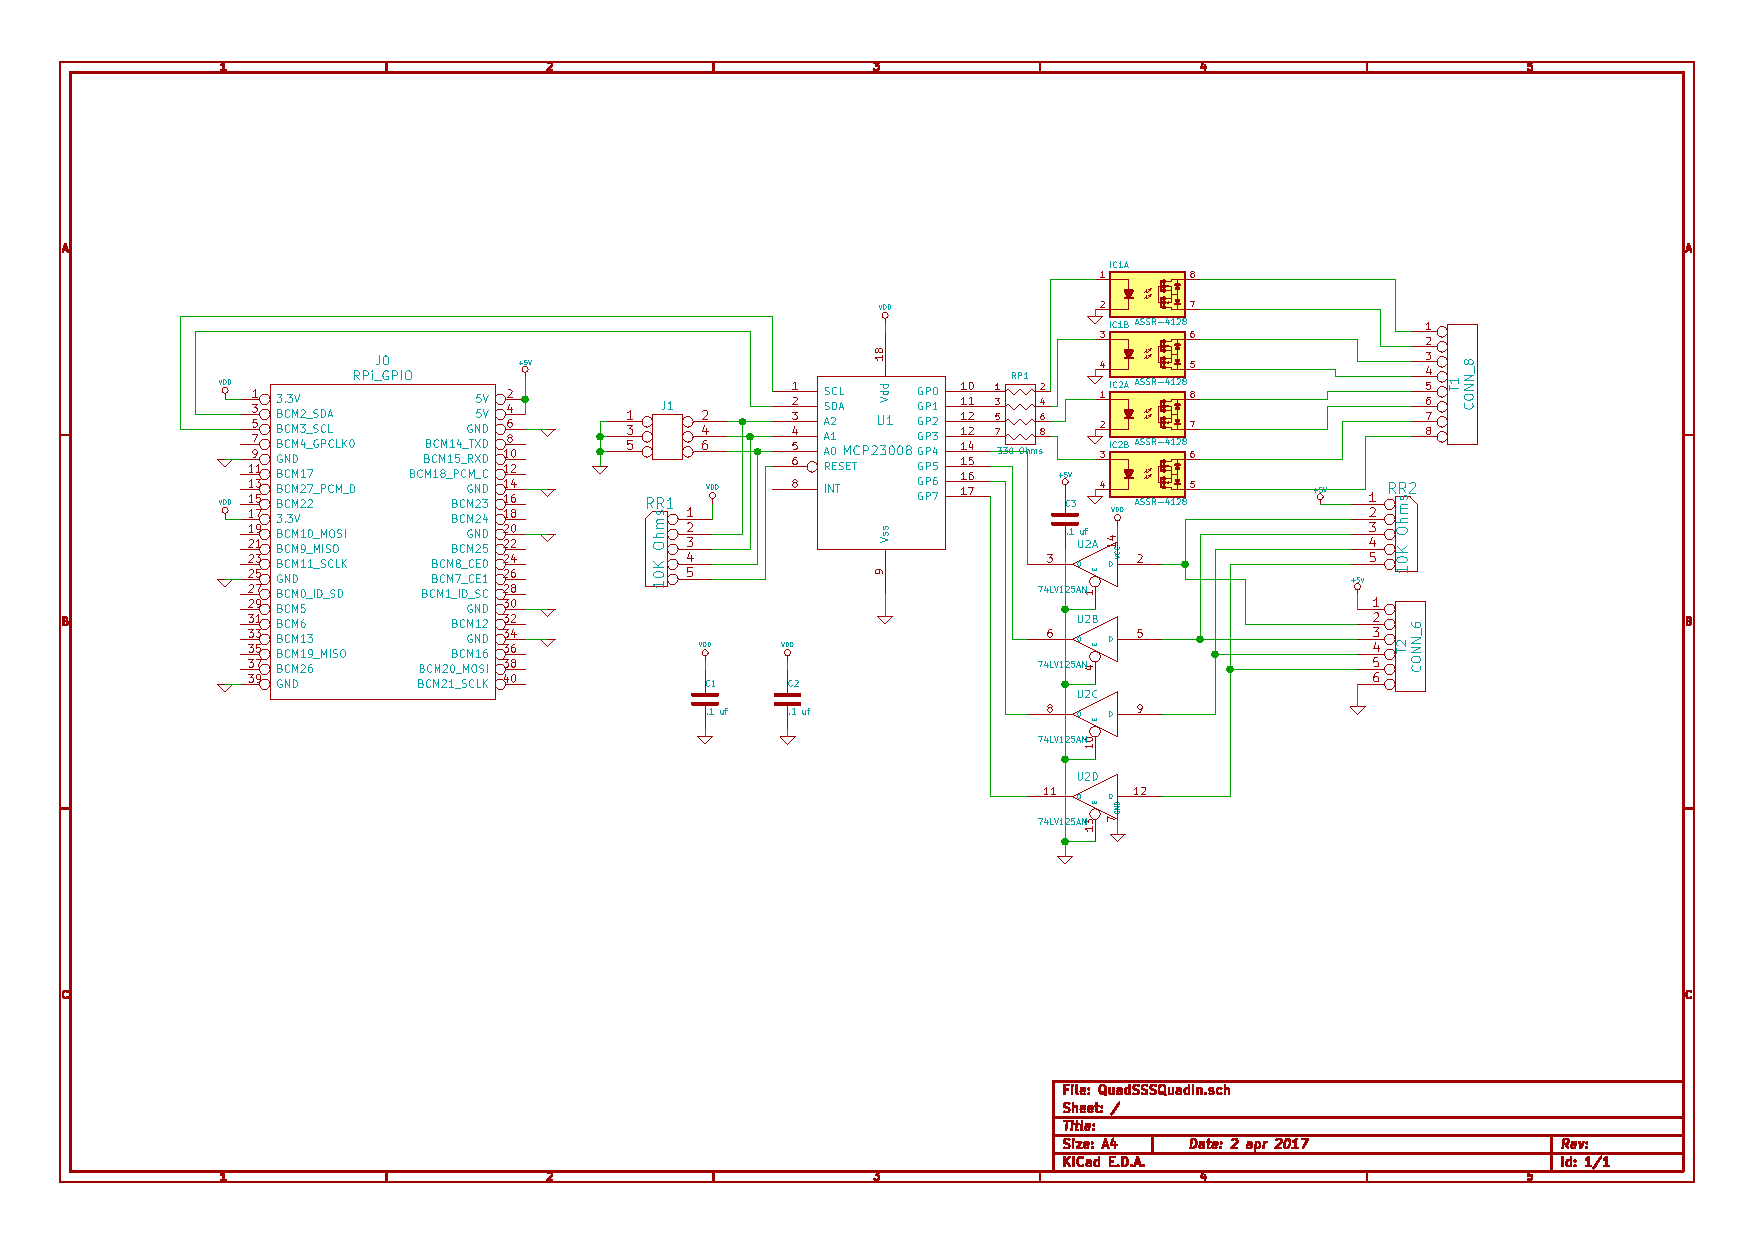
\includegraphics[width=5in]{QuadSSSQuadIn.pdf}
\caption{Circuit Diagram of the QuadSSSQuadIn}
\end{centering}\end{figure}
This circuit uses a MCP23008 to expand the Raspberry Pis I/O to 8 additional 
I/O pins.  Four of these pins (0-3) are used to drive a pair of dual 
opto-isolated SSR chip and the remaining 4 (4-7) are driven by a input buffer 
chip that can be driven with 5V logic.  The SSRs can be used to switch 
arbitrary trackside devices, since the output side of the SSRs are rated upto 
+/- 400 volts at up to 0.1 Amp (100ma).  The 5V logic inputs are compatible 
with many sensor boards available (particularly occupancy detector circuits).

\section{Parts List}

\begin{table}[htdp]
\begin{centering}\begin{tabular}{|l|l|p{1in}|l|p{.5in}|}
\hline
Value&Qty&Refs&Mouser Part Number&Adafruit Part Number\\
\hline
.1 uf&3&C1 C2 C3&21RZ310-RC&\\
\hline
ASSR-4128&2&IC1 IC2&630-ASSR-4128-002E&\\
\hline
RPi GPIO&1&J0&855-M20-6102045&2223\\
\hline
CONN 3X2&1&J1&517-929836-02-03&\\
\hline
330 Ohms&1&RP1&652-4608X-AP2-331LF&\\
\hline
10K Ohms&2&RR1 RR2&652-4605X-1LF-10K&\\
\hline
CONN 8&1&T1&651-1725711&\\
\hline
CONN 6&1&T2&651-1725698&\\
\hline
MCP23008&1&U1&579-MCP23008-E/P&\\
\hline
74LV125AN&1&U2&595-SN74LV125AN&\\
\hline
\end{tabular}
\caption{Parts list for QuadSSSQuadIn boards.}
\end{centering}\end{table}\footnote{Mouser Project link: 
\url{http://www.mouser.com/ProjectManager/ProjectDetail.aspx?AccessID=97fe7b85dc}.}

The only parts that might be substituted are J0 (the RPi GPIO Header), and T1
and T2 (the I/O terminals). The parts listed are for the stacking headers for 
the RPi GPIO Header, and screw terminals for the I/O terminals.  Feel free to 
select a non-stacking header for the RPi GPIO Header and to select either pin 
arrays or spring terminals for the T1 and T2.                   

\section{Circuit Board Layout}

\begin{figure}[hbpt]\begin{centering}%
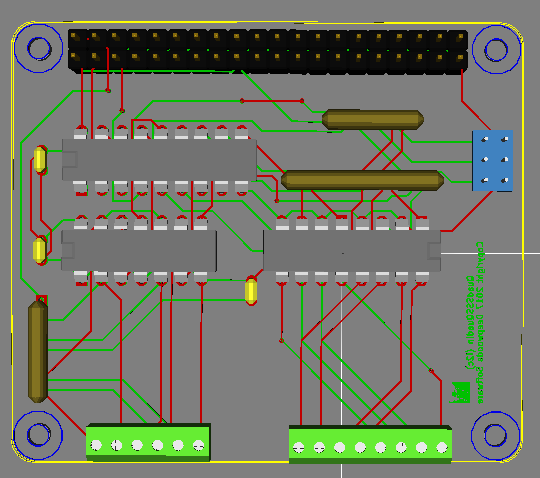
\includegraphics[width=5in]{QuadSSSQuadIn3DTop.png}
\caption{3D rendering of the QuadSSSQuadIn board}
\end{centering}\end{figure}
\begin{figure}[hbpt]\begin{centering}%
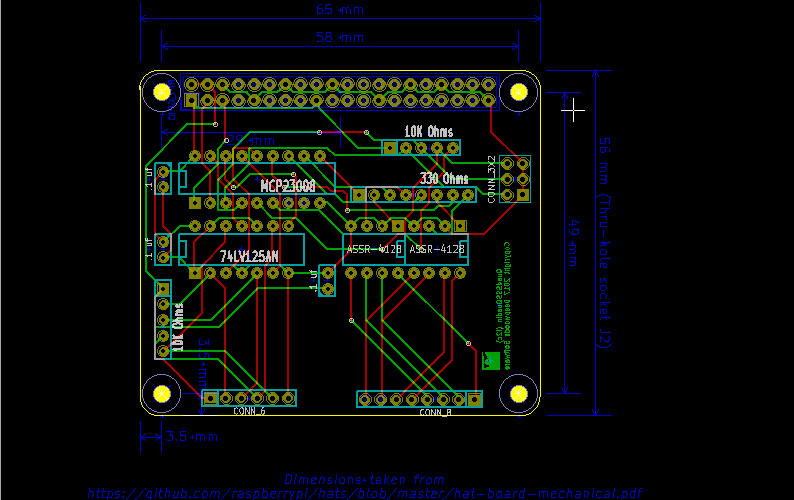
\includegraphics[width=5in]{QuadSSSQuadIn.png}
\caption{Fabrication image of the QuadSSSQuadIn board}
\end{centering}\end{figure}
Board assembly is straight forward.  You need to be careful orienting the ICs, 
noting that the SSRs are oppositely oriented from the other ICs.  Also the 
SIP resistor arrays need to be carefully oriented -- the dot marks pin 1, 
which is indicated on the board with a square pad\footnote{The first batch of 
the boards I ordered used the wrong PCB modules for the terminals and the 
holes are too small for the screw terminal pins to go all the way in.  They 
can be ``jammed'' in enough to be soldered. Pin arrays fit a little better, 
but still need some effort to seat.  The next batch I order will not have this 
problem.}. 

\section{Downloadables and Software Support}

Full design information is available on GitHub here:
\url{https://github.com/RobertPHeller/RPi-RRCircuits/tree/master/QuadSSSQuadIn}.

This board is supported by the Model Railroad System
\texttt{OpenLCB\_PiMCP23008} daemon. A basic XML file for it is included in 
its GitHub folder. 

